%first_line
\documentclass[11pt]{article} % letterpaper is american!

\usepackage[british,UKenglish,USenglish,english,american]{babel}
\usepackage[pdftex]{graphicx}
\usepackage{epstopdf}

\usepackage{amsfonts,amsmath,amsthm,amssymb}

%\usepackage[T1]{fontenc}

\usepackage{tikz,pgf}
\usetikzlibrary{fit}

\pagestyle{empty}
\setlength{\parindent}{0mm}
\usepackage[letterpaper, margin=0.7in]{geometry}
%\usepackage{showframe}

\usepackage{multicol}
\usepackage{enumerate}

\usepackage{color}
\usepackage{verbatim}
\usepackage{listings}
\lstset{
  basicstyle=\scriptsize\ttfamily,
  backgroundcolor=\color{lightgray},
  language=bash,
  frame=L,
}


\usepackage{xspace}
\usepackage{url}
\usepackage{cite}

\usepackage{titlesec}
\titlespacing*{\subsubsection}{0pt}{*0}{*0}
\titlespacing*{\subsection}{0pt}{0pt}{*0}
\titlespacing*{\section}{0pt}{0pt}{*0}

\newcommand{\Bold}{\mathbf}


\setlength{\parskip}{1em}
\setlength{\parindent}{1em}

\def\ptk{peval-toolkit\xspace}
\def\ppaml{PPAML\xspace}

\title{New Documentation for PPAML-Eval-Tools}

\date{\today}

\author{Philip Robinson}

\newenvironment{mitemize}[1]{
  \begin{minipage}{\columnwidth}
  \subsubsection*{#1}
  \begin{itemize}
    \setlength{\topsep}{0pt}
    \setlength{\itemsep}{1pt}
    \setlength{\parsep}{0pt}
    \setlength{\parskip}{0pt}
}{\end{itemize}\end{minipage}}

\begin{document}
\pagestyle{empty}
\clearpage\maketitle

  \section*{Goals and Requirements}

  It is our goal to provide a \ptk that allows for us to human-efficiently compute and store quantitative metrics for team submissions to the \ppaml program. In this most recent submissions iteration, there was a significant amount of time that lost to setup, configuration, queuing executions of challenge problem solutions, and querying team status's. 

    We have been asked by the teams to provide a more rigid acceptance criteria. To aid in this, we are making our execution model more transparent. Although we don't want the teams to use relative paths, we are going to provide for them the following expectation of execution.

\begin{multicols}{2}
\begin{lstlisting}
$ tree -p ${ROOT}

tmp.IPT7bqEaJQ/
|-- [drwxrwxr-x]  conf/
|   |-- [-rw-rw-r--]  pref.conf
|   |-- [-rw-rw-r--]  smoke.conf
|-- [drwxrwxr-x]  engine/
|-- [-rwxrwxr-x]  env_setup.sh*
|-- [lr-xr-x---]  indata -> /path/to/data
|-- [drwxrwxr-x]  outdata/
|-- [drwxrwxr-x]  solution/
|-- [drwxrwxr-x]  tmp/

5 directories, 4 files
$
\end{lstlisting}
\vfill\columnbreak
\begin{lstlisting}
$ cat ${ROOT}/env_setup.sh 
#!/bin/bash -eu

export ROOT=`readlink -m $(dirname $0)`
# mkdir -p ${ROOT}/{engine,solution,tmp}

export ENGINE=${ROOT}/engine
export SOLUTION=${ROOT}/solution
export TMP=${ROOT}/tmp
$
\end{lstlisting}
\end{multicols}

\section*{Use Cases}
\begin{multicols}{2}

\begin{mitemize}{TA2-4}
  \item team submits PPS
  \item team submits CPS
\end{mitemize}

\begin{mitemize}{TA1}
  \item add team
  \item add challenge problem
  \item add definition to challenge problem
  \item add evaluator to definition
\end{mitemize}

\begin{mitemize}{TA1-2-4}
  \item add CPS or PPS
  \item add dataset to definition
  \item run solution
  \item evaluate solution
  \item query solution/team status
  \item generate report
\end{mitemize}

\end{multicols}

\newpage
\section*{Work-flow}
By better discussing the intended work-flow we can outline the changes that need to be applied to the present \ptk.

\subsection*{Terminal}

\begin{multicols}{2}
  \subsubsection*{Present}
  The ini files being addressed/created do not correctly allow for separation of PPS and CPS. Many of the submissions were delivered such that separation of the PPS from CPS is not possible. This prevents us from performing progress comparisons.

  There were also no tools for querying the database for valid input variables, so teams must know their id values without help (or by using sql queries).

  % We do not presently enfource any restrictions on time or memory usage. 
  
  The present model could be extended to have a cps.ini, pps.ini, and eval.ini files. but this becomes unmanageable quickly, it may be better to have conf.ini that is updated as states are accomplished.  

  % We do not have a trivial way of tagging 
  We need to include reporting tools, database updating/merging, and sample data in the released versions of the \ptk.
  
  \begin{lstlisting}
# create ini file to manually populate only
#   corresponds to cp-solutions
$ ppaml init <team-id> <challenge-id> 

# run solution as defined by ini file
$ ppaml run <cps.ini>

# evaluate output from run execution
$ ppaml eval <cps.ini>

# reports are externally executed and directly 
#   querey the database
$ ./generate_reports.py 
  \end{lstlisting}
  
  \vfill\columnbreak
  \subsubsection*{Goal}
  Instead of 'team' owning 'pps-type' owning 'pps-instances' it makes sense to just make 'team' representative of pps-type which owns engines\footnote{To increase clarity, I am decoupling the term 'pps' and 'engine'.}
  \begin{lstlisting}
# provide list operations
$ ppaml list teams
$ ppaml list problems

# engines listed by date and population
$ ppaml list engines <team-id> 
  \end{lstlisting}
  We frequently didn't know the status of the teams and challenge problem wrt evaluations and runtime. It would be nice to have a simple  tool to report run\_id date eval(\#t/\#f) runtime information.
  \begin{lstlisting}
# provide simple table
$ ppaml status teams
$ ppaml status problems
  \end{lstlisting}

  We will now treat the ini file as a descriptor to a user state machine. This will require that any artifact also contains a baseline ini file.
  \begin{lstlisting}
# to create a baseline ini file we should only
#   need team-id (pps-id seems redundtant)
$ ppaml use team <team-id> -output <conf.ini>

# manually populate with pps information
#   testing by build or check-install script
#   conf.ini will be stored in the artifact

# update and extend conf.ini to include
#   template challenge problem solution fields
$ ppaml use engine   --file <conf.ini> # OR
$ ppaml use engine   --id <engine-id>

# manually populate cps information including 
#   challenge problem id
$ ppaml use solution --file <conf.ini> # OR
$ ppaml use solution --id <solution-id>

# nothing to manually change
$ ppaml run solution --file <conf.ini> # OR
$ ppaml run solution --id <artifact-id> 5

# execute latest from each team
$ ppaml run <challenge-id>
  \end{lstlisting}
  \vfill
  \end{multicols}

  \subsection*{Sequence Diagram}

  The sequence diagram below designates what the intedned workflow of a submition from a team. 

  \begin{center}
    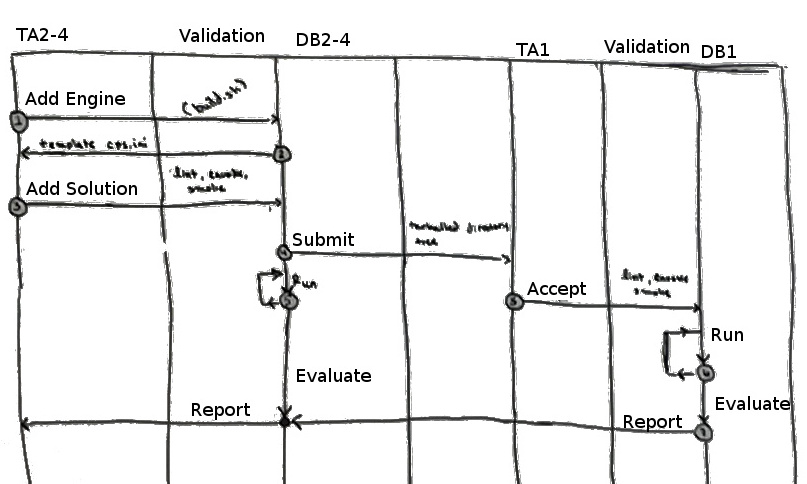
\includegraphics[width=0.9\textwidth]{sequence_diagram.jpg}
    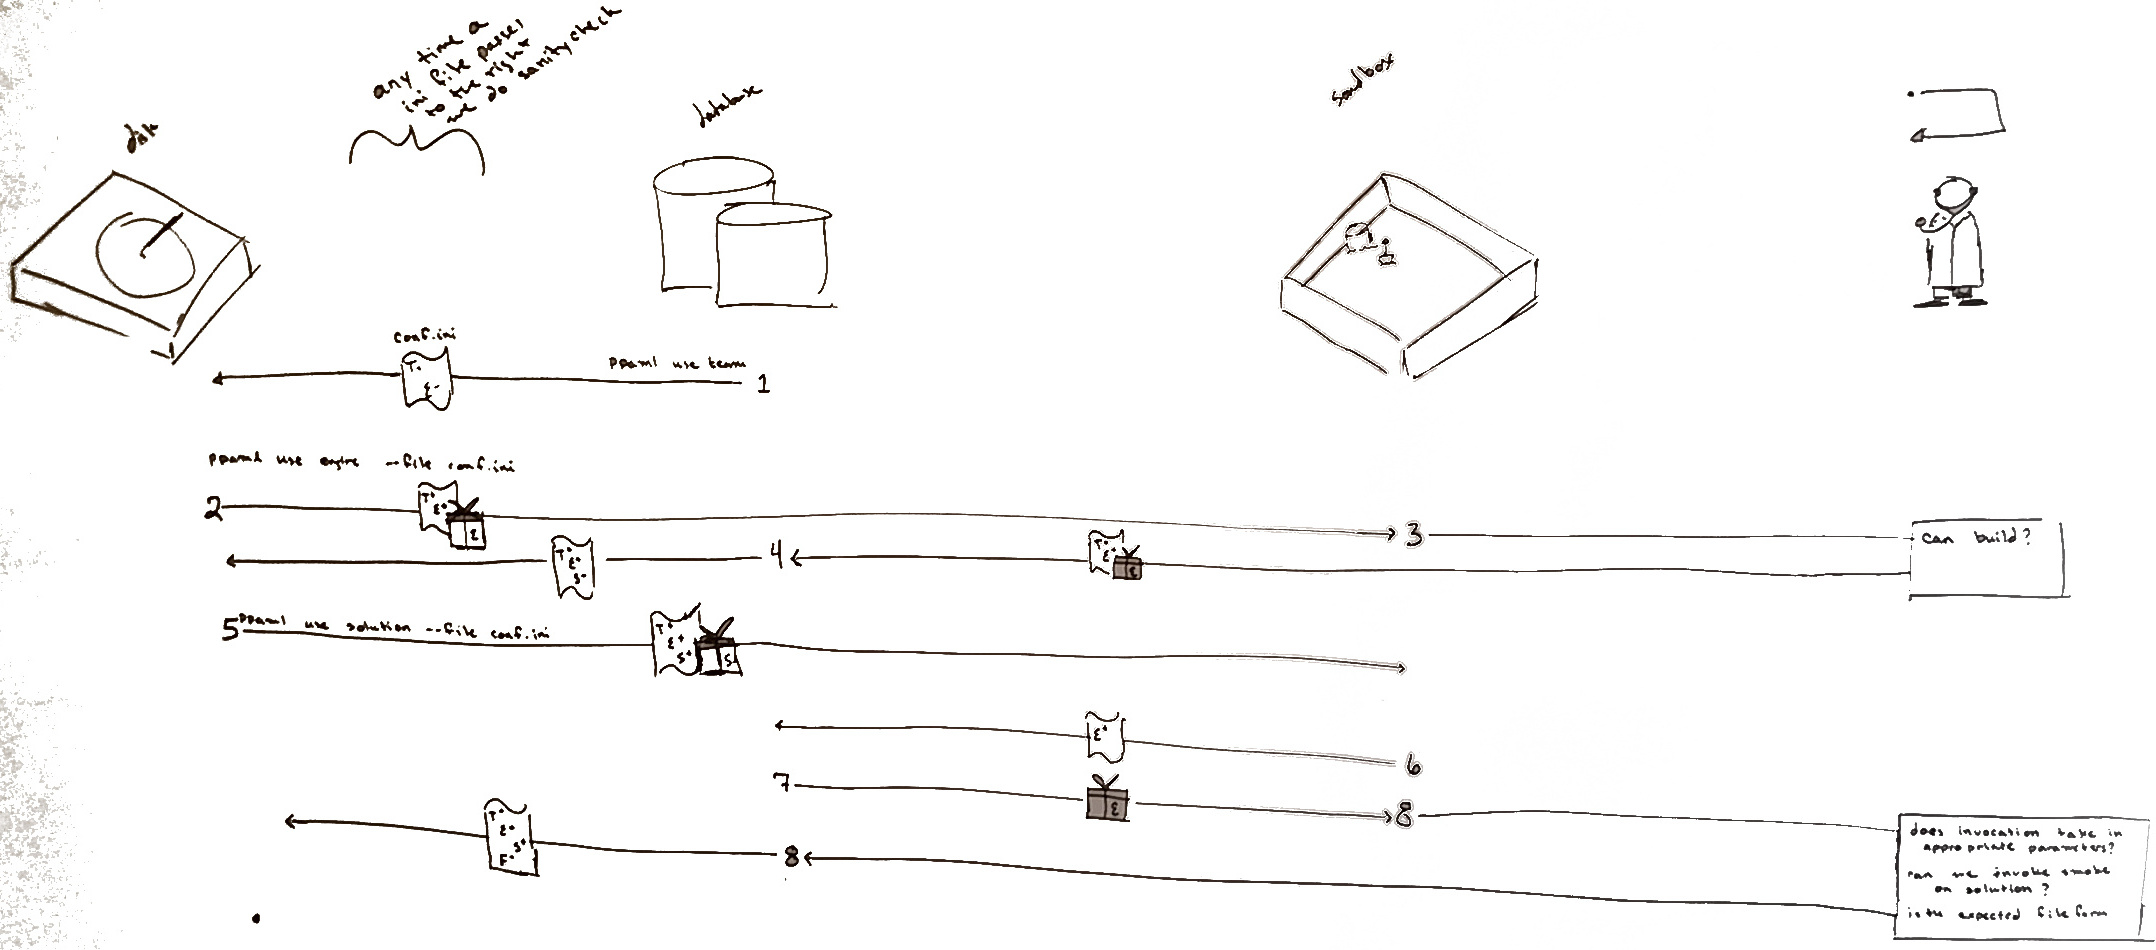
\includegraphics[width=0.9\textwidth]{more_sequence.jpg}
  \end{center}
  
  
  \newpage
\subsection*{Entity Relationship Diagram}
  \begin{center}
    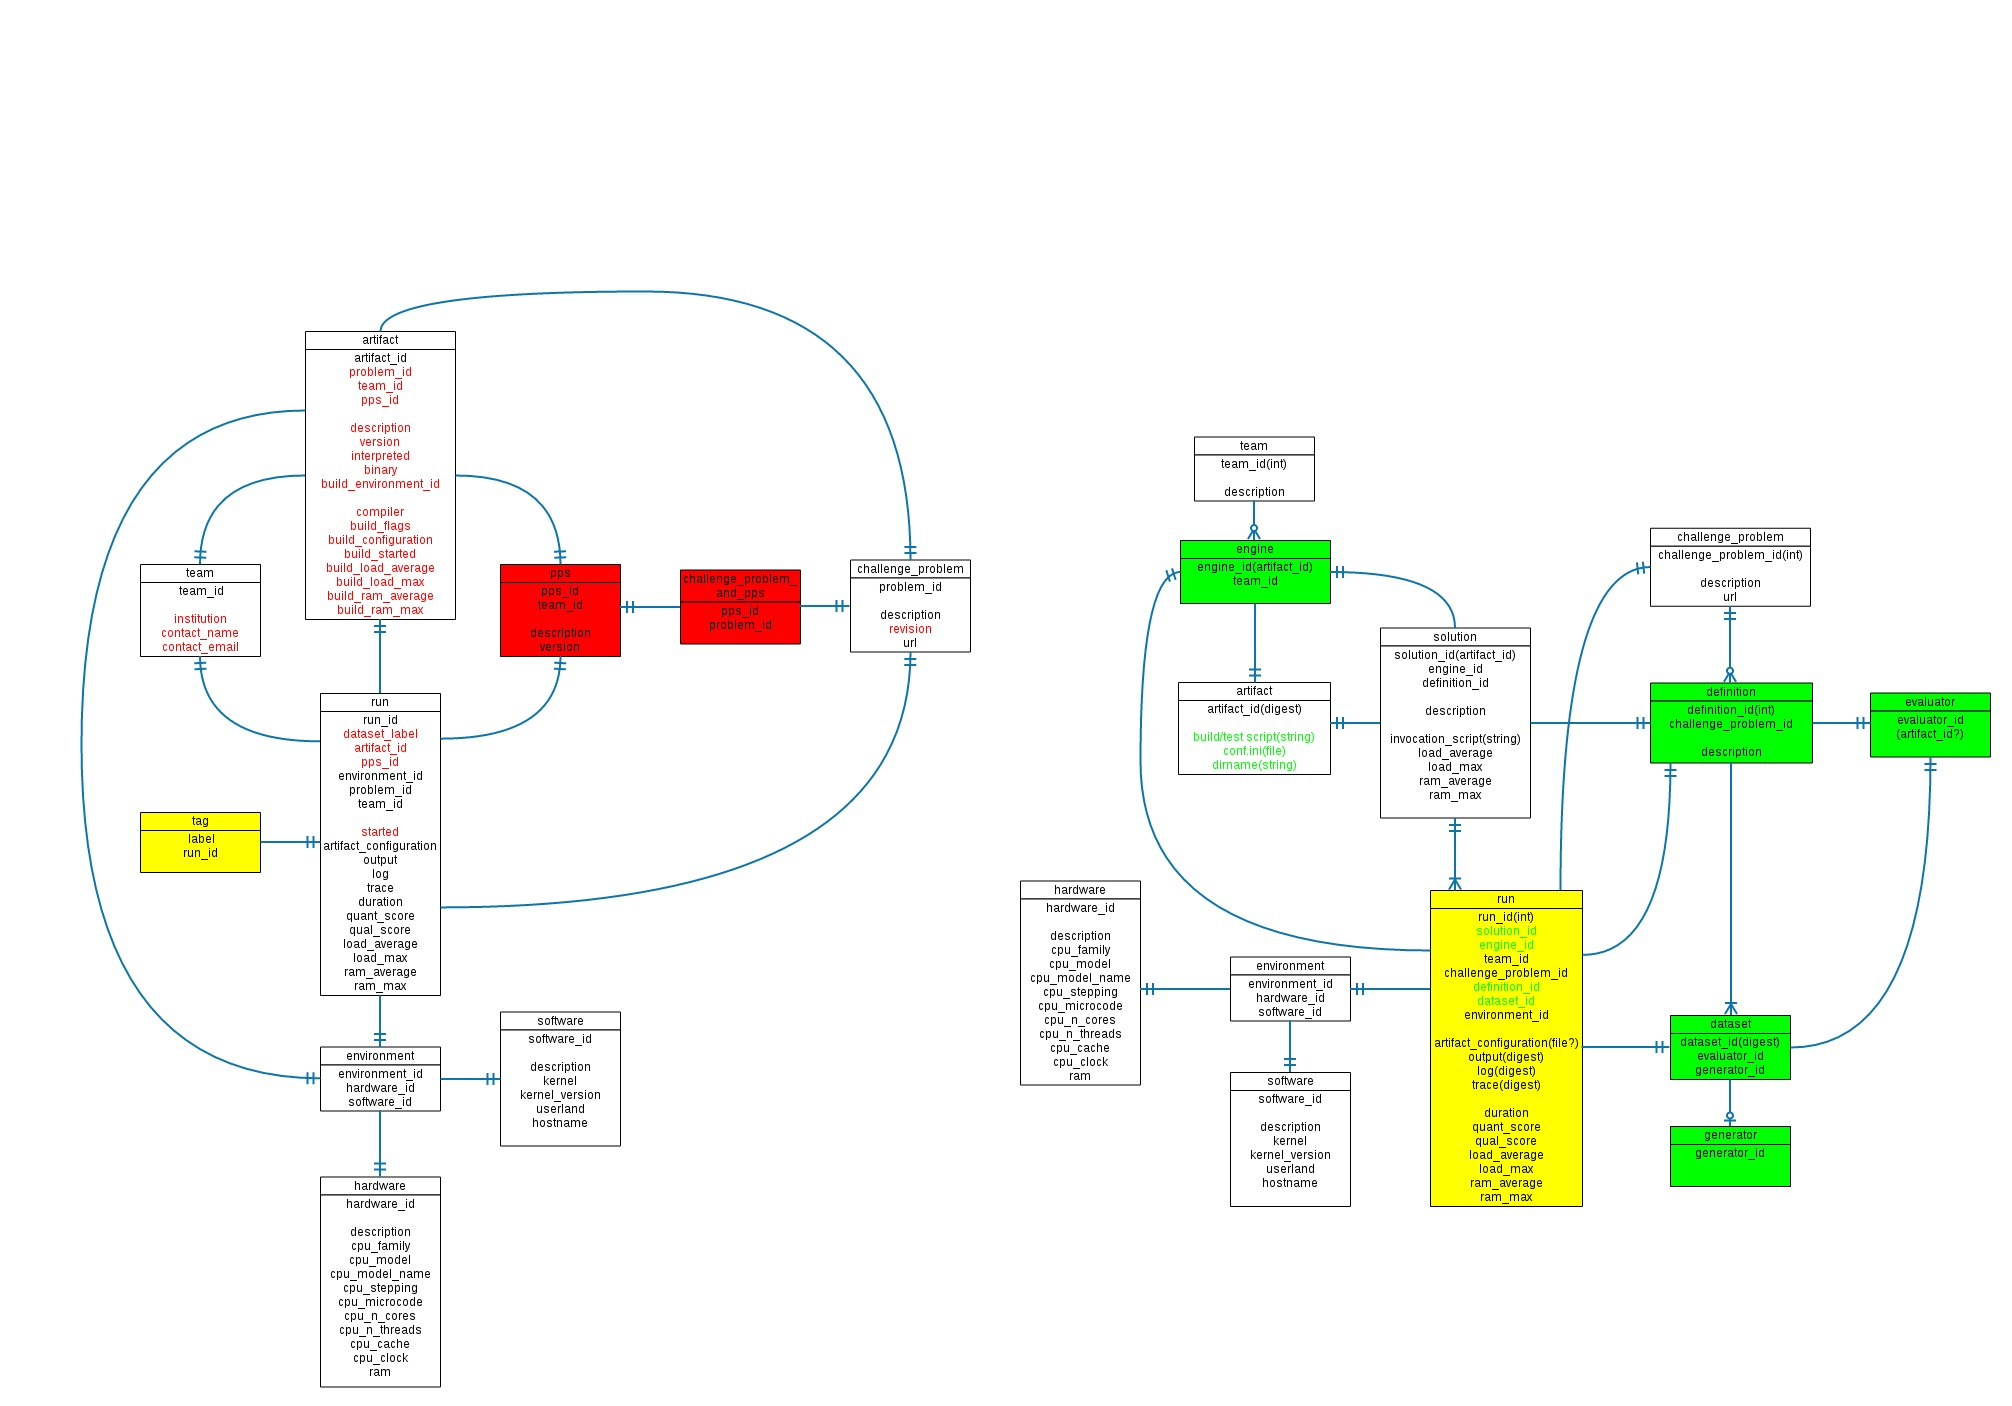
\includegraphics[width=\textwidth]{erd_ppaml.jpg}
    
    {\footnotesize just incase we need to edit this it was made with gliffy}
  \end{center}

  The changes above accomidate some of the challenges we faced, and some we are anticipating. There is likely some more room for editing. There is definately information that it doesnt really make sense to keep track of, like `contact information' for the teams and `build environment.'

  Open question may determine if datasets are to be `artifacted' or not.
\newpage
\section*{Present File Relations and Responsabilities}
\begin{multicols}{2}
{\centering \includegraphics[width=0.9\columnwidth]{peval.png}}

\begin{mitemize}{main}
\item initializes subparsers for argparse
\item handles messages from internal errors
\end{mitemize}

\begin{mitemize}{utility}
\item creates temporary directories for sandboxing
\item defines errors that are used from \ptk
\item directory digests for unique naming
\item message formating
\item tar and path operations
\end{mitemize}

\begin{mitemize}{db}
\item interface to sqlite using sqlalchemy {\em could likely be cleaned up to better support tagging}
\item triggers `migration' into and out of database using digests and utilities' sandboxing
\item defines object representation of tables in database
\item responsible for triggering `db\_init.sql' init.db DNE {\em we may want to better understand how to provide initial values, than rope insertion} 
\item {\em needs to be cleaned up a lot}%{\em ini information passed into and printed from print\_table\_info}
\end{mitemize}

\begin{mitemize}{evaluate}
\item process manager for executing evaluators
\item {\em evaluator grabbed from ini file instead of database}
\end{mitemize}

\begin{mitemize}{run}
\item process manager for executing solutions submissions
\item uses fingerprint and database
\item {\em no pps information is processed}
\item {\em needs to be cleaned up a lot}
\item {\em likely isn't profiling efficiently}
\end{mitemize}

\begin{mitemize}{ps}
\item defines ini operations and classes
\item used heavily to pass information through command line tools
\item {\em in every use is renamed `configuration' due to former name colision problem}
\end{mitemize}

\begin{mitemize}{add\_team}
\item adds record information describing teams to database
\item {\em new ERD implies that teams and PPS information are equivelent}
\end{mitemize}

\begin{mitemize}{add\_pps}
\item adds record information describing pps to database
\item {\em does not actually `artifact' the pps, only adds record information}
\end{mitemize}

\begin{mitemize}{tag}
\item simple CLI allowing tags of single runs with human readable name in database
\item {\em the primary goal of this file should be revisited}
\end{mitemize}

\begin{mitemize}{submit}
\item wrap up relevent artifacts to a run for submission
\item {\em only presently wraps up CPS instance, not dataset labels or pps}
\end{mitemize}

\begin{mitemize}{fingerprint}
\item profiles the system for RAM, operating system, and CPU
\item {\em requires patch on virtual machine, makes me feel this could be done better, however patch is uploaded as well so will likely be low priority}
\end{mitemize}

\begin{mitemize}{init}
\item responsible for providing the `ppaml init' command
\item provides empty ini file for manual population
\end{mitemize}
\end{multicols}
\begin{comment}
\newpage

\begin{enumerate}
  \item Still need class module diagrams
  \item talk to mike about submission process options
  \item list Questions for chris
  \item we need workflow for adding challenge problems and datasets to the database
  \item we need to revisit the intended purpose and implementation of tags
\end{enumerate}
\end{comment}
\end{document}
